\lecture[20]{20. Fyrsta stigs diffurjöfnur}{lecture-text}
\date{5.~nóvember 2012}

\title{\insertlecture}
\mode<presentation>
{
\author{%\begin{center}
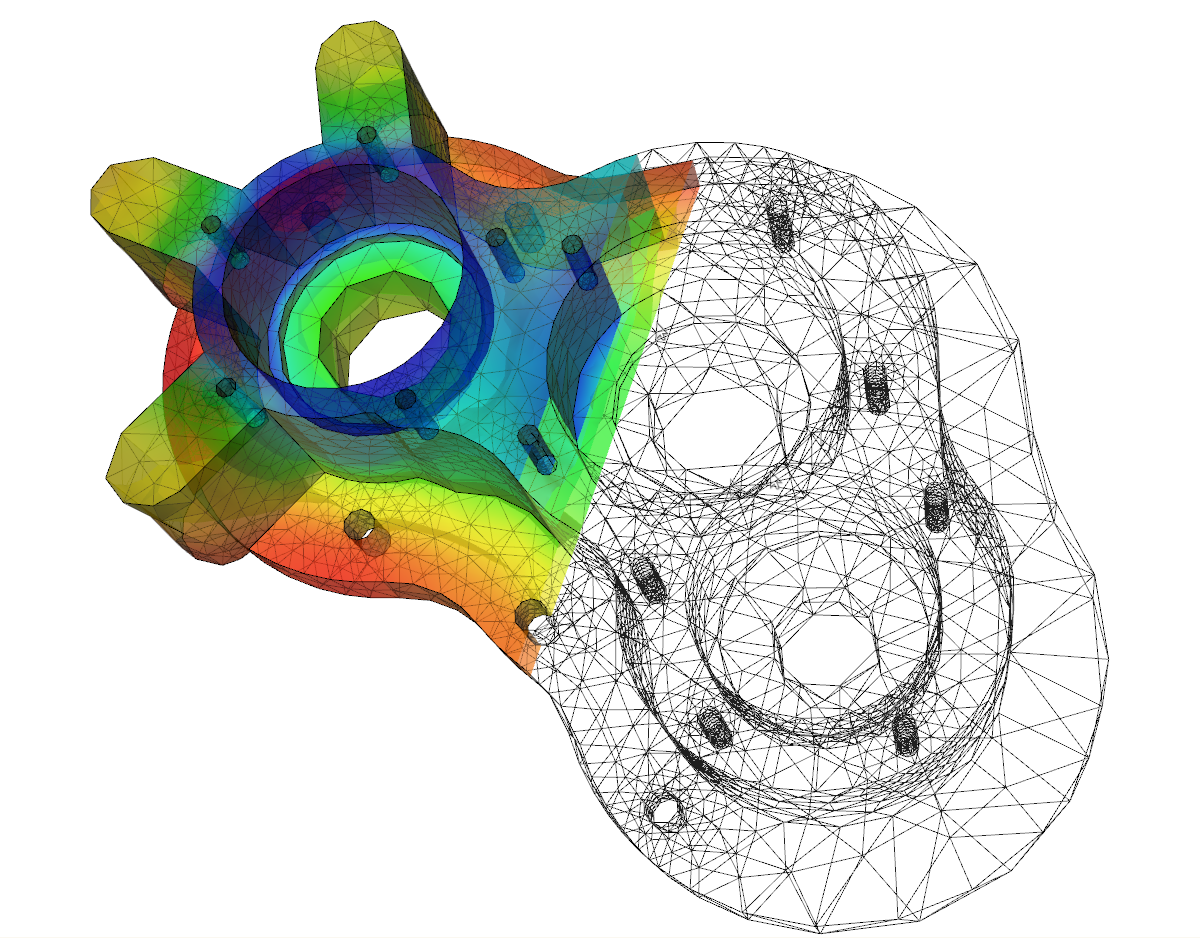
\includegraphics[width=5cm]{./myndir/IB11-f20_heat-equation.png}
%\end{center}
\\
Benedikt Steinar Magnússon, \href{mailto:bsm@hi.is}{bsm@hi.is}}
}

\begin{document}

\subsection[t]
	\maketitle
\mode<article>
{
\begin{center}
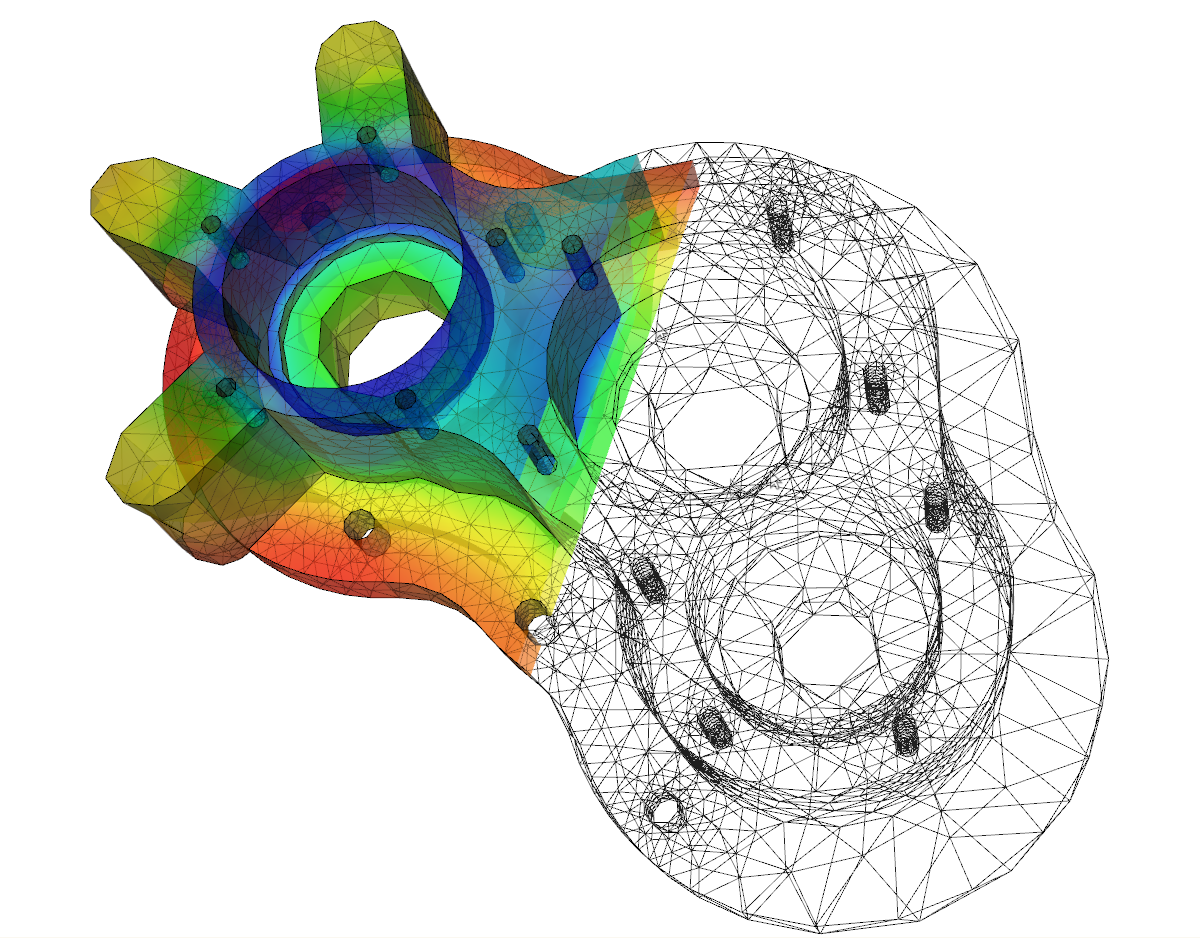
\includegraphics[width=5cm]{./myndir/IB11-f20_heat-equation.png}
\end{center}
}


\section*{}
\subsection[t]{Diffurjöfnur}
 \subsubsection{20.1 Skilgreining.}  Ritum $y=y(x)$ sem fall af $x$. \pause

{\em Diffurjafna} er jafna á forminu 
$$F(x, y, y', y'', \ldots, y^{(n)})=0$$
þar sem $F$ er fall (formúla) í $n+1$ breytistærð. \pause 

Jafnan er sögð
vera af $n$-ta {\em stigi} ef hæsta afleiða $y$ sem kemur fyrir í
formúlu er $n$.
 

\pause

\subsubsection{20.2 Dæmi}
 Það að finna stofnfall fyrir fall $f$ er jafngilt því að leysa 
fyrsta stigs diffurjöfnuna 
$$
y'(x) = f(x),
$$
\pause
eða með framsetningunni úr 20.1,
$$
F(x,y') = f(x) - y'(x) = 0.
$$




\subsection[t]{Aðgreinanlegar diffurjöfnur}
 \subsubsection{20.3 Aðgreinanlegar diffurjöfnur.} 
Fyrsta stigs diffurjafna sem má rita
á forminu 
$$\frac{dy}{dx}=f(x)g(y)$$ \pause
kallast {\em aðgreinanleg} (e. seperable).  \pause
Það er, þátta má hægri hliðina  þannig að annar þátturinn
er bara fall af $x$ og hinn þátturinn er bara fall af $y$.

\pause

Umritum jöfnuna yfir á formið 
$$\frac{dy}{g(y)}=f(x)\,dx.$$ \pause
\textbf{Athugið}: Ekkert $x$ í vinstri hlið, 
ekkert $y$ í hægri hlið. 
\pause

Síðan smellum við heildum á báðar hliðar og fáum að 
$$\int\frac{dy}{g(y)}=\int f(x)\,dx.$$
 


\subsection[t]{}
 \subsubsection{} 
Reiknum stofnföllin hægra og vinstra megin í jöfnunni
$$\int\frac{dy}{g(y)}=\int f(x)\,dx.$$
og munum eftir að setja inn heildunarfasta \pause
(einn er nóg).  \pause

Þá höfum við jöfnu sem tengir saman $x$ og $y$, og inniheldur engar
afleiður af $y$. \pause

Út frá þeirri
jöfnu má fá upplýsingar um eiginleika lausnarinnar $y$. \pause 

Stundum er hægt að einangra $y$ og fá þannig formúlu fyrir lausn diffurjöfnunar.
 


\subsection[t]{Línulegar diffurjöfnur}
 \subsubsection{20.4 Skilgreining.} 
Diffurjafna á forminu
$$a_n(x)y^{(n)}+a_{n-1}(x)y^{(n-1)}+\cdots+a_1(x)y'+a_0(x)y=f(x)$$
kallast {\em línuleg diffurjafna}. \pause
Hún er $n$-ta stigs ef $a_n(x)$ er
ekki fastafallið $0$.  \pause

Ef $f$ er fastafallið $0$ þá er jafnan sögð
{\em óhliðruð} (e. homogeneous) \pause en ef $f$ er ekki fastafallið $0$ þá
er hún sögð {\em hliðruð} (e. nonhomogeneous). 
 


\subsection[t]{Línulegar fyrsta stigs diffurjöfnur}
 \subsubsection{20.5 Línulegar fyrsta stigs diffurjöfnur.}
Almenna línulega fyrsta stigs jöfnu má rita á forminu
$$y'+p(x)y=q(x).$$

\pause
Samsvarandi óhliðruð jafna er
$$y'+p(x)y=0.$$

\pause
Skilgreinum $\mu(x)=\int p(x)\,dx$ (eitthvert stofnfall).  Þá er 
$$y(x)=e^{-\mu(x)}\int e^{\mu(x)}q(x)\,dx$$
lausn á diffurjöfnunni.  


\pause

\subsubsection{Athugasemd}
Þegar þið reiknið $\mu(x)=\int p(x)\,dx$ þá
megið þið sleppa heildunarfastanum, en \textbf{ekki} þegar þið reiknið heildið 
$\int e^{\mu(x)}q(x)\,dx$.
 


\subsection[t]{Samantekt}
 \subsubsection{Aðskiljanlegar jöfnur}
 Jöfnur sem hægt er að rita á forminu
 $$
 \frac{dy}{dx} = f(x)g(y),
 $$
 má leysa með því að heilda og einangra $y$ út úr
 $$
 \int \frac 1{g(y)}\, dy = \int f(x)\, dx.
 $$
 
 \pause
 \subsubsection{Línulegar fyrsta stigs jöfnur}
	 Lausn við jöfnu á forminu 
	 $$
		y'(x) + p(x)y = q(x)
	$$
	er gefin með 
	$$
	y(x) = e^{-\mu(x)} \int e^{\mu(x)} q(x)\, dx,
	$$
	þar sem $\mu(x) = \int p(x)\, dx$.
 





\end{document}
\lecture[21]{21. Annars stigs diffurjöfnur}{lecture-text}
\date{7.~nóvember 2012}


\begin{document}

\subsection
	\maketitle


\section*{}
\subsection[t]{Línulegar annars stigs diffurjafnur með
  fastastuðla}
 \subsubsection{21.1 Skilgreining}  {\em Línuleg annars stigs diffurjafna með
  fastastuðla} er diffurjafna á forminu 
$$ay''+by'+cy=f(x)$$
þar sem $a, b$ og $c$ eru fastar. \pause

Jafnan er sögð {\em óhliðruð}
(e. homogeneous) ef fallið $f(x)$ er fastafallið 0. 
 

\pause

 \subsubsection{21.2 Skilgreining} Jafnan $ar^2+br+c=0$ kallast \emph{kennijafna}
(e. auxiliary equation)
diffurjöfnunnar $ay''+by'+cy=0$.
 


\subsection[t]{Línulegar samantektir lausna}
 \subsubsection{21.3 Setning}  Ef föllin $y_1(x)$ og $y_2(x)$ eru lausnir á
diffurjöfnunni $ay''+by'+cy=0$ þá er fallið
$$y(x)=Ay_1(x)+By_2(x),$$  
þar sem $A$ og $B$ eru fastar, líka lausn. 

\pause

Ef $y_2(x)$ er ekki
fastamargfeldi af $y_1(x)$ þá má skrifa \textbf{sérhverja} lausn $y(x)$ á
diffurjöfnunni $ay''+by'+cy=0$ á forminu
$$y(x)=Ay_1(x)+By_2(x),$$  
þar sem $A$ og $B$ eru fastar.
 


\subsection[t]{Lausn óhliðraðar annars stigs línulegrar diffurjöfnu með
  fastastuðla}
 \subsubsection{21.4 Setning}
\begin{description}
\item[Tilvik I] \emph{Kennijafnan $ar^2+br+c=0$ hefur tvær ólíkar rauntölulausnir
  $r_1$ og $r_2$.}

\pause
Fallið
$$y(x)=Ae^{r_1x}+Be^{r_2x}$$
er alltaf lausn sama hvernig fastarnir $A$ og $B$ eru valdir og
sérhverja lausn má rita á þessu formi.

\pause

\item[Tilvik II] \emph{Kennijafnan $ar^2+br+c=0$ hefur bara eina rauntölulausn
  $k=-\frac{b}{2a}$.}

\pause

Fallið
$$y(x)=Ae^{kx}+Bxe^{kx}$$
er alltaf lausn sama hvernig fastarnir $A$ og $B$ eru valdir og
sérhverja lausn má rita á þessu formi.
\end{description}
 


\subsection[t]{
\mode<presentation>{
Lausn óhliðraðar annars stigs línulegrar diffurjöfnu með
  fastastuðla, framhald
}
}
 \subsubsection{
\mode<presentation>{
21.4. Setning, framhald}
}
\begin{description}
\item[Tilvik III] \emph{Kennijafnan $ar^2+br+c=0$ hefur engar rauntölulausnir.}

\pause

Setjum $k=-\frac{b}{2a}$ og $\omega=\frac{\sqrt{4ac-b^2}}{2a}$. \pause

Rætur kennijöfnunnar eru $r_1=k+i\omega$ og $r_2=k-i\omega$.
\pause

Fallið
$$y(x)=Ae^{kx}\cos(\omega x)+Be^{kx}\sin(\omega x)$$
er alltaf lausn sama hvernig fastarnir $A$ og $B$ eru valdir \pause og
sérhverja lausn má rita á þessu formi.
\end{description}
 


\subsection[t]{Lausn hliðraðar annars stigs línulegrar diffurjöfnu með
  fastastuðlum}
 \subsubsection{21.5 Setning}
Látum $y_{\rm p}(x)$ vera einhverja lausn á hliðruðu jöfnunni
  $$
ay''+by'+cy=f(x).
$$ 
\pause

Látum $y_1(x)$ og $y_2(x)$ vera lausnir sem fást úr 21.4 á
  óhliðruðu jöfnunni
$$
ay''+by'+cy=0.
$$

\pause

Sama hvernig fastarnir $A$ og
  $B$ eru valdir þá er fallið 
$$y(x)=Ay_1(x)+By_2(x)+y_{\rm p}(x)$$ \pause
alltaf lausn á diffurjöfnunni  $ay''+by'+cy=f(x)$ og sérhverja lausn
má skrifa á þessu formi.
 


\subsection[t]{Ágiskanir}
 \subsubsection{21.6 Ágiskanir} (Sjá ramma í grein 17.6)

Leysa á jöfnu $ay''+by'+cy=f(x)$.

\pause

Látum $P_n(x)$ standa fyrir einhverja $n$-ta stigs margliðu og látum
$A_n(x)$ og $B_n(x)$ tákna $n$-ta stigs margliður með óákveðnum stuðlum. 

\begin{itemize}
\item Ef $f(x)=P_n(x)$ þá giskað á $y_{\rm p}(x)=x^mA_n(x)$.
\item Ef $f(x)=P_n(x)e^{rx}$ þá giskað á $y_{\rm p}(x)=x^mA_n(x)e^{rx}$.
\item Ef $f(x)=P_n(x)e^{rx}\sin(kx)$ 
þá giskað á $y_{\rm p}(x)=x^me^{rx}[A_n(x)\cos(kx)+B_n(x)\sin(kx)]$.
\item Ef $f(x)=P_n(x)e^{rx}\cos(kx)$ 
þá giskað á $y_{\rm p}(x)=x^me^{rx}[A_n(x)\cos(kx)+B_n(x)\sin(kx)]$.
\end{itemize} \pause
Hér táknar $m$ minnstu töluna af tölunum 0, 1, 2 sem tryggir að enginn
liður í ágiskuninni sé lausn á óhliðruðu jöfnunni $ay''+by'+cy=0$.

 

% 
% \subsection[t]{}
%  \subsubsection{}
%  
%  
% 
% 
% \subsection[t]{}
%  \subsubsection{}
%  
%  
% 



\end{document}
